\documentclass[twocolumn]{article}
\usepackage[margin=0.6in]{geometry}

\usepackage[small,compact]{titlesec}

\usepackage{graphicx}
\usepackage{listings}
\usepackage{color}
\usepackage{hyperref}


\title{COMP 6360 Wireless and Mobile Networks \\ Project 1 Report}
\author{Team 2\thanks{Jiao Yu [jzy0012], Song Gao [szg0031], Xinyu Que [xzq0003] (ordered by name)}}
\date{Mar. 7, 2012}

\begin{document}

\maketitle

\section{Architecture}
\par{The simulator consists of three threads and multiple classes. As shown in Figure~\ref{fig:arch}, they work collaboratively to simulate the EEBL application. Section~\ref{sec:design} discusses details of each part of the system.}
\begin{figure}[htb]
    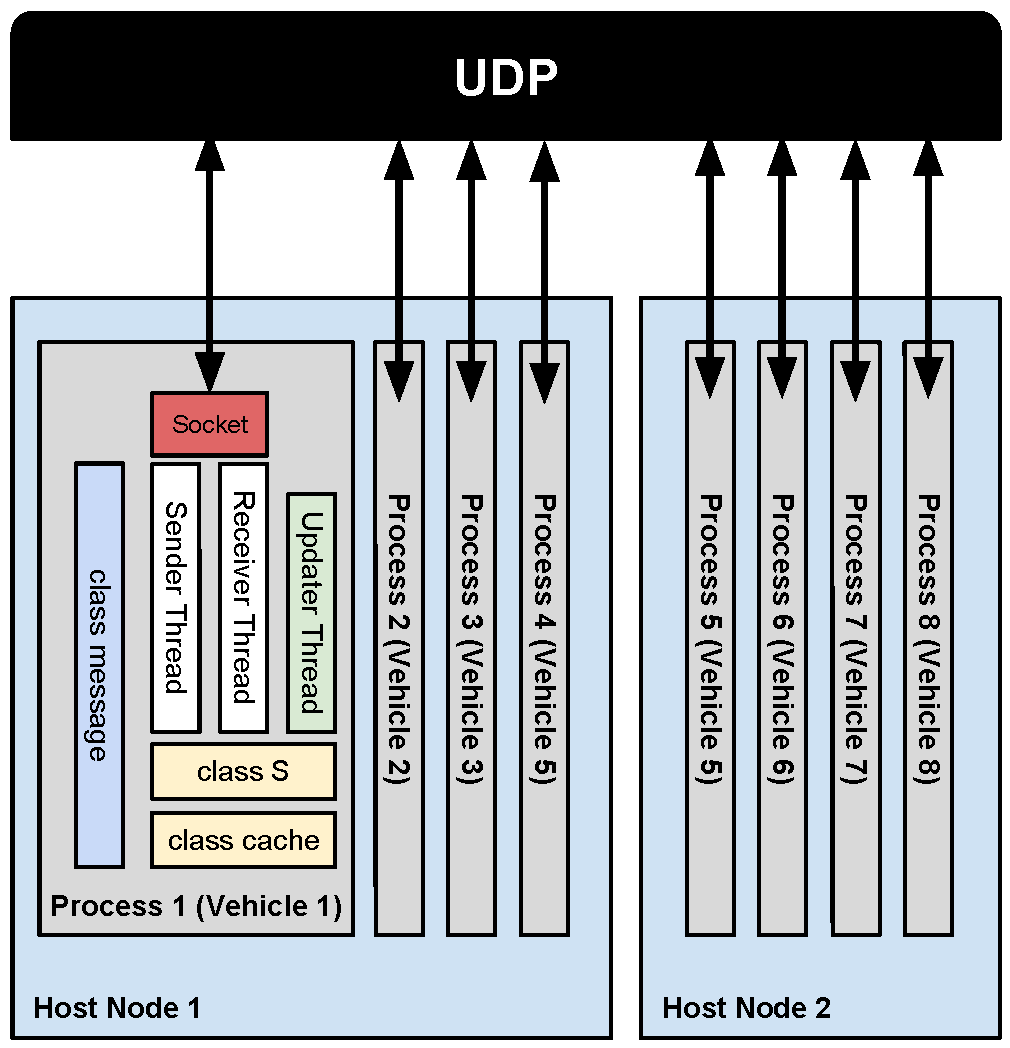
\includegraphics[width=\columnwidth]{fig_arch.pdf}
    \caption{Architecture}
    \label{fig:arch}
\end{figure}

\section{Design}
\label{sec:design}
\subsection{Message modeling and serialization}
{\bf Involved classes: } {\tt message, vehicle}
\par{{\tt message} class is in charge of modeling and manipulating messages. It has three main responsibilities:}
\subsubsection{Carrying Data}
\par{We use a same message structure for both beacons and EEBL messages. It takes 46 bytes in amount. Table~\ref{tab:data} shows information carried by {\tt message} class.}
\begin{table}[htb]
    \begin{tabular}{|r|c|r|c|r|c|}
        \hline  
        {\bf Data}      & {\bf Size}    & {\bf Data}            & {\bf Size}    \\ \hline
        Message Type    &   1           & Vehicle Heading       &   2           \\ \hline
        Packet ID       &   4           & Vehicle Size          &   6           \\ \hline
        Originator ID   &   4           & Vehicle Speed         &   2           \\ \hline
        Sender ID       &   4           & Vehicle Acceleration  &   2           \\ \hline
        Time-to-live    &   1           & GPS Coordinate        &   12          \\ \hline
        Timestamp       &   8           &                       &               \\ \hline
    \end{tabular}
    \caption{Message Format}
    \label{tab:data}
\end{table}
\par{Since vehicle IDs and packet IDs have same size (4 bytes), we have to suppose that packet IDs are unique in a single vehicle, however, different vehicles may have identical packet IDs. Therefore, vehicle ID and packet ID combined together can be used as unique packet identifier in the whole network.}
\subsubsection{Build Messages}
\par{In addition to carrying data, {\tt message} class is also capable of creating three kind of messages: BEACON, EEBL, and Rebroadcasted EEBL. It automatically accomplishes some of message operations that are not dependent on upper layer code. For example, it updates TTL when rebroadcasting EEBL message; and it retrieves static vehicle informations such as vehicle ID/heading. It is designed to make upper-layer code provide as little extra data as possible when creating messages.}
\subsubsection{Serialization and Deserialization}
Finally, {\tt message} class also provides interface to manipulate byte stream which is used by sockets to transmit over UDP. Two methods, 
\begin{lstlisting}[language=C++,keywordstyle=\color{blue}]
static message * message::from_bytes(
        const unsigned char data[]);
void message::to_bytes(
        unsigned char buffer[])const;
\end{lstlisting}
, are implemented to transform between byte array and message object. By encapsulation lower-layer functions like {\tt memcpy}, it enables upper-layer code to only deal with structured data.
\subsection{Concurrent Data Share}

\par{In some situations, multiple concurrent threads need to share data and synchronize operations. For example, we have an application-layer thread(Section~\ref{sec:thread_updater}) to update vehicle state such as speed and acceleration, and (in the future) to determine whether collision will take place. This thread needs to share data with sending thread and receiving thread, which deal with socket communication.}
\par{To avoid corrupted data operation, {\tt S} class, a thread-safe singleton class, is implemented. {\tt S} ensures that only one instance exists in a process. It stores data that needs to be available globally to multiple threads, and use locking mechanism to synchronize concurrency operations in different threads. We choose {\tt std::mutex} and {\tt std::lock\_guard} from {\tt C++0x} to implement locks. Lock guarded data includes {\it GPS coordinate, speed, acceleration, EEBL message queue}. In addition to these shared state data, a thread-safe cache(see Section~\ref{sec:class_cache} for details) is also accessible via {\tt S} class.}
\par{{\tt S} class is initialized at the beginning of {\tt main} function. It takes configuration file path and node number as arguments, and pass them to {\tt configuration} class constructor(see Section~\ref{sec:class_configuration} for details) during initialization phase.}
\subsection{Fast Cache For Messages and EEBL Identifiers}
\label{sec:class_cache}
\par{{\tt cache} class implements a simple cache that stores recently received messages(including both BEACON and EEBL) and unique identifiers of recently received EEBL. The former one indicates state of other vehicles, which is used to calculate distance-based rebroadcasting probability as well as predicting collision, etc., while the later one is used to determine a certain rebroadcasted EEBL message has already been received before. To make it thread-safe, a locking mechanism similar to {\tt S} class is used.}
\par{To achieve good performance for both data retrieval/replacement and inserted-time-based removal, {\tt cache} class uses hash tables ({\tt std::unordered\_map/std::unordered\_set}) to store the actual data, and binary search trees ({\tt std::multimap}) to index the stored data by timestamp. In this way, data is accessible from hash tables with high performance, and since indexes are sorted on timestamp, removing outdated items can be accomplished via index very fast. Currently, we set alive time for messages and EEBL identifiers to be 8 seconds and 4 seconds.}
\subsection{{\tt configuration} class Design}
\par{Reading data from the configuration file is encapsulated by the configuration class. The configuration file in our project has the format of “Node 1 tux175 10120 links 2 GPS 120 225”, which basically means Node 1 is simulated by tux175 with port number 10120,and connected to Node 2, also its GPS coordinate is (120, 225). The Configuration class builds three maps (implemented by C++ STL) for recording the $<tux\#, port\#>$ pair, linked nodes number as a vector, and GPS coordinate as a struct with keys node number. It provides three services to its clients, which returns the pointers to the three maps.}
\subsection{Threads Implementation}
\par{We split the program into 3 threads, 
\begin{lstlisting}[language=C++,keywordstyle=\color{blue}]
void * sender_main(void * context)
void * recver_main(void * context)
void * updater_main(void * context)
\end{lstlisting}
, to do the job of sending packets, receiving packets, and updating acceleration/deceleration and speed of vehicles respectively . In the following subsections, more details of each thread are discussed.}
\subsubsection{Sender Thread}
\par{First of all, the sender thread should know which nodes are within its communication range, and get their tux machine name and port numbers from the configuration file. Then a UDP socket is created, and the socket addresses of its neighboring nodes are converted from machine names and ports. There are 3 types of packets need to be sent, EEBL originated by the node itself, EEBL to be rebroadcasted, and beacon packets. The node will continuously check whether its deceleration is greater than 1m/s, which necessitates generating and sending original EEBL signal. Here we use a third thread—the updater thread, to randomly pick a acceleration of -2m/s with p = 0.2, or 2m/s with p = 0.8. For rebroadcast EEBL packets, the sender thread will check a global queue, which contains the EEBL packets that the node decides to rebroadcast according to a probability model. The queue will be filled by receiver thread, and the probability model will be discussed further in the receiver thread section. We set the priority of original EEBL packets and rebroadcast EEBL packets to be the same, which precedes beacon packets. }
\subsubsection{Receiver Thread}
\par{The receiver thread is responsible for receiving packets and making the decision of whether to rebroadcast a new EEBL packet. To do this job, the receiver thread first needs to get its own tux machine name and port number from the configuration file and convert it to socket address. Then it will create a UDP socket and bind that socket to its own socket address. Upon receiving a packet, the thread is going to first check the type of that packet, EEBL or beacon. If it is a EEBL packet, the receiver needs to know whether it is old or new by looking up the cache. Old packets will just be ignored and deleted, while new EEBL packets will be processed by the rebroadcast protocol. In our project, we use a probability model for rebroadcasting shown in Eq.~\ref{eq:prob}. }
\begin{equation}
    P=(\frac{distance}{communication range})^3
    \label{eq:prob}
\end{equation}
\par{After calculating the rebroadcasting probability for a new EEBL packet, the receiver would generate a uniformly distributed random number between 0 and 1. If the random number is less than P, then this packet is going to be rebroadcasted, and will be put in the queue for the sender thread to pull rebroadcasting packets out. Also the new EEBL packets would be put in cache no matter it is going to be rebroadcasted or not. If a beacon message is received, then it is simply put in cache. Our cache is designed in such a way that it can handle both EEBL and beacon packets, maintain an index of them based on in-cache timestamp, and delete expired packets automatically.}
\subsubsection{Updater Thread}
\label{sec:thread_updater}
\par{The updater thread is responsible for simulating the change in a vehicle’s acceleration and speed. For the purpose of simplicity, we set the node’s acceleration to only take two values, -2m/s or 2m/s, with probability 0.2 and 0.8 respectively, with an updating frequency of 10Hz. Speed will be updated according to the random acceleration.}
\subsection{Main Function}
\par{Main function function contains threads, namely send thread, receive thread and update thread. Send thread sends beacon message with a fixed frequency and receive thread receives beacon messages. Once receive thread receives EEBL messages, it will inform sender to broadcast EEBL messages. Update thread is to simulate the break of vehicle with a certain probability.}
\subsection{Makefile}
\par{Makefile stores compiler and linker options and expresses all the interrelationships among source files. (A source code file needs specific include files, an executable file requires certain object modules and libraries, and so forth.) Make program reads the makefile and then invokes the compiler, assembler, resource compiler, and linker to produce the final output, which is generally an executable file. The make program uses built-in inference rules that tell it, for example, to invoke the compiler to generate an OBJ file from a specified CPP file.}
\subsection{Launch script}
\par{A launch script is written to automatically launch the programs across many host machines, which provides a very easy and efficient way to start the program and analyze the results. In our program, the bash script first reads the {\tt conf} file and gets the nodes information. Then it sequentially log in to host machines and launch the programs. }
\label{sec:class_configuration}

\begin{thebibliography}{9}
    \bibitem {segata11} Michele Segata and Renato Lo Cigno. 2011. {\it Emergency braking: a study of network and application performance.} In Proceedings of the Eighth ACM international workshop on Vehicular inter-networking (VANET '11). ACM, New York, NY, USA, 1-10. DOI=10.1145/2030698.2030700 http://doi.acm.org/10.1145/2030698.2030700
    \bibitem {eeblr} O. Tonguz, N. Wisitpongphan, J. Parikh, F. Bai, P. Mudalige, and V. Sadekar. {\it On the Broadcast Storm Problem in Ad hoc Wireless Networks.} In Broadband Communications, Networks and Systems, 2006. BROADNETS 2006. 3rd International Conference on, pages 1–11, Oct. 2006.
    \bibitem {c++0xthreading} Anthony Williams. {\it Simpler Multithreading in C++0x.} \url{http://www.devx.com/SpecialReports/Article/38883/1954}
\end{thebibliography}
\end{document}

